\documentclass[12pt,letterpaper]{article}
\usepackage[latin1]{inputenc}
\usepackage[spanish]{babel}
\usepackage{amsmath}
\usepackage{amsfonts}
\usepackage{amssymb}
\usepackage{graphicx}
\usepackage[hidelinks]{hyperref}
\usepackage{color}
\graphicspath{{Imagenes/}}
\usepackage[left=2cm,right=2cm,top=2cm,bottom=2cm]{geometry}
\author{M�rquez M�rquez Amairani Ivette}
\begin{document}
\begin{center}
\textbf{\huge{Universidad Politecnica de la Zona \\[0.5cm] Metropolitana de Guadalajara}}
\end{center}

\begin{center}

\includegraphics[width=0.65\textwidth]{Imagenes/UPCDLZMDG5783-logo.png}\\[2cm] 
\end{center}
\vspace{0.1cm}
{\large\textbf{Evidencia:} 2.8 Calcular los parametros de circuitos activos de transistores de \\potencia\\[0.2cm]\textbf{Alumno:} M�rquez M�rquez Amairani Ivette\\[0.2cm]\textbf{Profesor:} Mor�n Garabito Carlos Enrique\\[0.2cm]\textbf{Carrera:} Ing. Mecatronica\\[0.2cm]\textbf{Grupo:} 4�B\\[0.2cm]\textbf{Fecha de entrega:} 29 de Octubre del 2019\\[0.2cm]}\\

\vspace{10cm}
\textbf{2.8 Calcular los par�metros de circuitos activos de transistores}\\[0.3cm]
El funcionamiento y utilizaci�n de los transistores de potencia es id�ntico al de los transistores normales, teniendo como caracter�sticas especiales las altas tensiones e intensidades que tienen que soportar y, por tanto, las altas potencias a disipar.\\
Existen tres tipos de transistores de potencia:\\[0.2cm]
\begin{itemize}
\item Bipolar.
\item Unipolar o FET (Transistor de Efecto de Campo).
\item IGBT.\\
\end{itemize}
En la Figura 1.Bipolar se muestra cierta comparaci�n entre un MOSFET y un transistor Bipolar.

\begin{figure}[h]
\centering
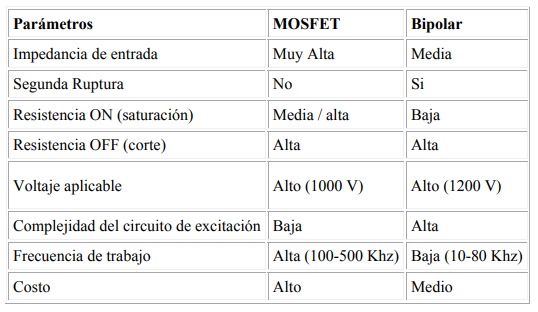
\includegraphics[width=0.50\textwidth]{Imagenes/Bipolar.PNG} 
\caption{Tabla comparativa}
\label{fig:tabla}
\end{figure}
 A continuaci�n se vera el siguiente ejemplo para calcular los par�metros de un transistor de potencia bipolar. (Observe el siguiente circuito en la Figura 2)

\begin{figure}[h]
\centering
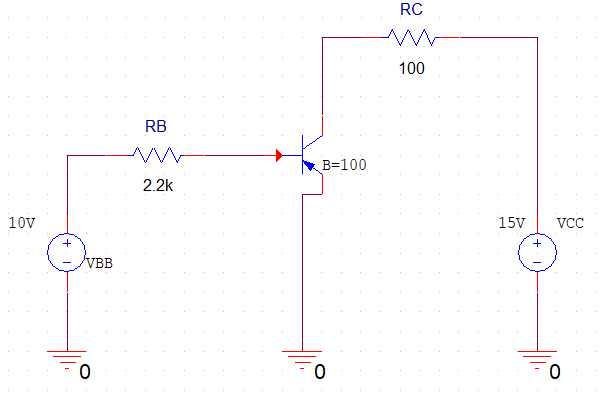
\includegraphics[width=0.50\textwidth]{Imagenes/Circuito.PNG}  
\caption{Circuito Bipolar}
\label{fig:Bipolar}
\end{figure}
\vspace{10cm}
\textbf{C�lculos:}\\[0.2cm]
$$I(sa) = \dfrac{Vcc}{Rc} $$

$$Vce=0 $$

$$Vce(corte)\approx Vcc $$

\textbf{Regla general:} $$Ib > \dfrac{Ic}{\beta} $$

$$-VBB + Ib \cdot Rb + 0.7V = 0$$

$$Ib = \dfrac{VBB-0.7V}{Rb}=\dfrac{10V-0.7V}{2.2k\Omega}=4.2mA$$

$$I(sa) = \dfrac{15V}{100\Omega} = 150mA$$

 $$Vce(corte)=15V$$
 
 $$\dfrac{Ic}{\beta}=\dfrac{150mA}{100}=1.5mA $$
 
 \textbf{Comprobaci�n:}\\[0.2cm]
 $$Ib > \dfrac{Ic}{\beta} = 4.2mA > 1.5mA $$
 
\vspace{2cm}
 {\large\textbf{Bibliograf�a}\\[0.2cm]

  \emph{Instituto N.C. Breage(Martes 21 de Agosto 2018). Transistores de potencia bipolar.}
 Obtenido de:
 \textcolor{blue}{ https://www.incb.com.mx/index.php/curso-de-electronica/95-curso-de-electronica-de-potencia/2633-curso-de-electronica-de-potencia-parte-3-transistores-de-potencia-bipolares-cur2003s}\\[0.3cm]

 \emph{Bermudez A.L(Julio 2018). Transistores de potencia.}
 Obtenido de:
 \textcolor{blue}{ http://www.profesormolina.com.ar/electronica/componentes/transist/pot.htm}\\[0.3cm]
\end{document}